% -*- Mode:TeX -*-

%% IMPORTANT: The official thesis specifications are available at:
%%            http://libraries.mit.edu/archives/thesis-specs/
%%
%%            Please verify your thesis' formatting and copyright
%%            assignment before submission.  If you notice any
%%            discrepancies between these templates and the 
%%            MIT Libraries' specs, please let us know
%%            by e-mailing thesis@mit.edu

%% The documentclass options along with the pagestyle can be used to generate
%% a technical report, a draft copy, or a regular thesis.  You may need to
%% re-specify the pagestyle after you \include  cover.tex.  For more
%% information, see the first few lines of mitthesis.cls. 

%\documentclass[12pt,vi,twoside]{mitthesis}
%%
%%  If you want your thesis copyright to you instead of MIT, use the
%%  ``vi'' option, as above.
%%
%\documentclass[12pt,twoside,leftblank]{mitthesis}
%%
%% If you want blank pages before new chapters to be labelled ``This
%% Page Intentionally Left Blank'', use the ``leftblank'' option, as
%% above. 

\documentclass[12pt,twoside]{mitthesis}
\usepackage{lgrind}
%% These have been added at the request of the MIT Libraries, because
%% some PDF conversions mess up the ligatures.  -LB, 1/22/2014
\usepackage{cmap}
\usepackage[T1]{fontenc}
\usepackage{graphicx}
\usepackage{hyperref}
\usepackage{listings}
\pagestyle{headings}

%% This bit allows you to either specify only the files which you wish to
%% process, or `all' to process all files which you \include.
%% Krishna Sethuraman (1990).

% \typein [\files]{Enter file names to process, (chap1,chap2 ...), or `all' to
% process all files:}
% \def\all{all}
% \ifx\files\all \typeout{Including all files.} \else \typeout{Including only \files.} \includeonly{\files} \fi

\begin{document}

% -*-latex-*-
% 
% For questions, comments, concerns or complaints:
% thesis@mit.edu
% 
%
% $Log: cover.tex,v $
% Revision 1.8  2008/05/13 15:02:15  jdreed
% Degree month is June, not May.  Added note about prevdegrees.
% Arthur Smith's title updated
%
% Revision 1.7  2001/02/08 18:53:16  boojum
% changed some \newpages to \cleardoublepages
%
% Revision 1.6  1999/10/21 14:49:31  boojum
% changed comment referring to documentstyle
%
% Revision 1.5  1999/10/21 14:39:04  boojum
% *** empty log message ***
%
% Revision 1.4  1997/04/18  17:54:10  othomas
% added page numbers on abstract and cover, and made 1 abstract
% page the default rather than 2.  (anne hunter tells me this
% is the new institute standard.)
%
% Revision 1.4  1997/04/18  17:54:10  othomas
% added page numbers on abstract and cover, and made 1 abstract
% page the default rather than 2.  (anne hunter tells me this
% is the new institute standard.)
%
% Revision 1.3  93/05/17  17:06:29  starflt
% Added acknowledgements section (suggested by tompalka)
% 
% Revision 1.2  92/04/22  13:13:13  epeisach
% Fixes for 1991 course 6 requirements
% Phrase "and to grant others the right to do so" has been added to 
% permission clause
% Second copy of abstract is not counted as separate pages so numbering works
% out
% 
% Revision 1.1  92/04/22  13:08:20  epeisach

% NOTE:
% These templates make an effort to conform to the MIT Thesis specifications,
% however the specifications can change.  We recommend that you verify the
% layout of your title page with your thesis advisor and/or the MIT 
% Libraries before printing your final copy.
\title{A Feedback System for Baseball Swings}

\author{Gerzain Mata}
% If you wish to list your previous degrees on the cover page, use the 
% previous degrees command:
%       \prevdegrees{A.A., Harvard University (1985)}
% You can use the \\ command to list multiple previous degrees
%       \prevdegrees{B.S., University of California (1978) \\
%                    S.M., Massachusetts Institute of Technology (1981)}
\department{Department of Electrical Engineering and Computer Science}

% If the thesis is for two degrees simultaneously, list them both
% separated by \and like this:
% \degree{Doctor of Philosophy \and Master of Science}
\degree{Bachelor of Science in Electrical Engineering and Computer Science}

% As of the 2007-08 academic year, valid degree months are September, 
% February, or June.  The default is June.
\degreemonth{June}
\degreeyear{2016}
\thesisdate{May 9, 2016}

%% By default, the thesis will be copyrighted to MIT.  If you need to copyright
%% the thesis to yourself, just specify the `vi' documentclass option.  If for
%% some reason you want to exactly specify the copyright notice text, you can
%% use the \copyrightnoticetext command.  
%\copyrightnoticetext{\copyright IBM, 1990.  Do not open till Xmas.}

% If there is more than one supervisor, use the \supervisor command
% once for each.
\supervisor{Jacob K. White}{Professor}

% This is the department committee chairman, not the thesis committee
% chairman.  You should replace this with your Department's Committee
% Chairman.
%\chairman{Arthur C. Smith}{Chairman, Department Committee on Graduate Theses}

% Make the titlepage based on the above information.  If you need
% something special and can't use the standard form, you can specify
% the exact text of the titlepage yourself.  Put it in a titlepage
% environment and leave blank lines where you want vertical space.
% The spaces will be adjusted to fill the entire page.  The dotted
% lines for the signatures are made with the \signature command.
\maketitle

% The abstractpage environment sets up everything on the page except
% the text itself.  The title and other header material are put at the
% top of the page, and the supervisors are listed at the bottom.  A
% new page is begun both before and after.  Of course, an abstract may
% be more than one page itself.  If you need more control over the
% format of the page, you can use the abstract environment, which puts
% the word "Abstract" at the beginning and single spaces its text.

%% You can either \input (*not* \include) your abstract file, or you can put
%% the text of the abstract directly between the \begin{abstractpage} and
%% \end{abstractpage} commands.

% First copy: start a new page, and save the page number.
\cleardoublepage
% Uncomment the next line if you do NOT want a page number on your
% abstract and acknowledgments pages.
% \pagestyle{empty}
\setcounter{savepage}{\thepage}
\begin{abstractpage}
% $Log: abstract.tex,v $
% Revision 1.1  93/05/14  14:56:25  starflt
% Initial revision
% 
% Revision 1.1  90/05/04  10:41:01  lwvanels
% Initial revision
% 
%
%% The text of your abstract and nothing else (other than comments) goes here.
%% It will be single-spaced and the rest of the text that is supposed to go on
%% the abstract page will be generated by the abstractpage environment.  This
%% file should be \input (not \include 'd) from cover.tex.


% In this thesis, I designed and implemented a compiler which performs
% optimizations that reduce the number of low-level floating point operations
% necessary for a specific task; this involves the optimization of chains of
% floating point operations as well as the implementation of a ``fixed'' point
% data type that allows some floating point operations to simulated with integer
% arithmetic.  The source language of the compiler is a subset of C, and the
% destination language is assembly language for a micro-floating point CPU.  An
% instruction-level simulator of the CPU was written to allow testing of the
% code.  A series of test pieces of codes was compiled, both with and without
% optimization, to determine how effective these optimizations were.

In this project, I designed and implemented a feedback system which samples roll, pitch, and yaw coordinates, saves them in nonvolatile memory, and provides the saved coordinates as desired values when performing feedback during replication attempts; this involves the sampling of an integrated accelerometer, gyroscope, and magnetometer unit, processing the raw measurements through an implementation of Madgwick's gradient descent filter, and storing floating point numbers in a ferroelectric RAM for later retrieval.  Feedback is given to the user through four vibration motors placed 90 degrees from each other along the main axis of the bat.  The construction of the swing feedback system involved the physical modification of a plastic bat, the addition of reinforcing members from laser-cut acrylic, the addition of LEDs and pushbuttons for user interaction, and the addition of four vibration motors.  The code incorporates open-source code available through GitHub and is based on the Arduino programming environment for accelerated embedded systems development.

\end{abstractpage}

% Additional copy: start a new page, and reset the page number.  This way,
% the second copy of the abstract is not counted as separate pages.
% Uncomment the next 6 lines if you need two copies of the abstract
% page.
% \setcounter{page}{\thesavepage}
% \begin{abstractpage}
% % $Log: abstract.tex,v $
% Revision 1.1  93/05/14  14:56:25  starflt
% Initial revision
% 
% Revision 1.1  90/05/04  10:41:01  lwvanels
% Initial revision
% 
%
%% The text of your abstract and nothing else (other than comments) goes here.
%% It will be single-spaced and the rest of the text that is supposed to go on
%% the abstract page will be generated by the abstractpage environment.  This
%% file should be \input (not \include 'd) from cover.tex.


% In this thesis, I designed and implemented a compiler which performs
% optimizations that reduce the number of low-level floating point operations
% necessary for a specific task; this involves the optimization of chains of
% floating point operations as well as the implementation of a ``fixed'' point
% data type that allows some floating point operations to simulated with integer
% arithmetic.  The source language of the compiler is a subset of C, and the
% destination language is assembly language for a micro-floating point CPU.  An
% instruction-level simulator of the CPU was written to allow testing of the
% code.  A series of test pieces of codes was compiled, both with and without
% optimization, to determine how effective these optimizations were.

In this project, I designed and implemented a feedback system which samples roll, pitch, and yaw coordinates, saves them in nonvolatile memory, and provides the saved coordinates as desired values when performing feedback during replication attempts; this involves the sampling of an integrated accelerometer, gyroscope, and magnetometer unit, processing the raw measurements through an implementation of Madgwick's gradient descent filter, and storing floating point numbers in a ferroelectric RAM for later retrieval.  Feedback is given to the user through four vibration motors placed 90 degrees from each other along the main axis of the bat.  The construction of the swing feedback system involved the physical modification of a plastic bat, the addition of reinforcing members from laser-cut acrylic, the addition of LEDs and pushbuttons for user interaction, and the addition of four vibration motors.  The code incorporates open-source code available through GitHub and is based on the Arduino programming environment for accelerated embedded systems development.

% \end{abstractpage}

\cleardoublepage

\section*{Acknowledgments}

Several individuals were instrumental in the realization of this project.  The workspace and equipment for this project were provided by the Cypress Engineering Design Studio along with the 6.302 lab workspace. Many thanks to the project supervisor, Professor Jacob K. White.  Sincere thanks to Joe Steinmeyer and Nick Arango for their recommendations in how to appropriately provide feedback to the user.  Many thanks to Gavin Darcey and the staff at the EDS for their assistance in using the laser cutter and their patience with the constant noise produced.  A special thank you to two students from the Electrical Engineering department: Hugo Malpica for your constant company and support in the development of this project.  Grant Gunnison for your words of encouragement and feedback in the development of this project.

%%%%%%%%%%%%%%%%%%%%%%%%%%%%%%%%%%%%%%%%%%%%%%%%%%%%%%%%%%%%%%%%%%%%%%
% -*-latex-*-

% Some departments (e.g. 5) require an additional signature page.  See
% signature.tex for more information and uncomment the following line if
% applicable.
 % % -*- Mode:TeX -*-
%
% Some departments (e.g. Chemistry) require an additional cover page
% with signatures of the thesis committee.  Please check with your
% thesis advisor or other appropriate person to determine if such a 
% page is required for your thesis.  
%
% If you choose not to use the "titlepage" environment, a \newpage
% commands, and several \vspace{\fill} commands may be necessary to
% achieve the required spacing.  The \signature command is defined in
% the "mitthesis" class
%
% The following sample appears courtesy of Ben Kaduk <kaduk@mit.edu> and
% was used in his June 2012 doctoral thesis in Chemistry. 

\begin{titlepage}
\begin{large}
This doctoral thesis has been examined by a Committee of the Department
of Chemistry as follows:

\signature{Professor Jianshu Cao}{Chairman, Thesis Committee \\
   Professor of Chemistry}

\signature{Professor Troy Van Voorhis}{Thesis Supervisor \\
   Associate Professor of Chemistry}

\signature{Professor Robert W. Field}{Member, Thesis Committee \\
   Haslam and Dewey Professor of Chemistry}
\end{large}
\end{titlepage}


\pagestyle{plain}
  % -*- Mode:TeX -*-
%% This file simply contains the commands that actually generate the table of
%% contents and lists of figures and tables.  You can omit any or all of
%% these files by simply taking out the appropriate command.  For more
%% information on these files, see appendix C.3.3 of the LaTeX manual. 
\tableofcontents
\newpage
\listoffigures
\newpage
%\listoftables


%% This is an example first chapter.  You should put chapter/appendix that you
%% write into a separate file, and add a line \include{yourfilename} to
%% main.tex, where `yourfilename.tex' is the name of the chapter/appendix file.
%% You can process specific files by typing their names in at the 
%% \files=
%% prompt when you run the file main.tex through LaTeX.
\chapter{Introduction}

Chapter two describes the design process, which includes the development of the enclosure and its modifications.

Chapter three describes the user input/output and a high-level overview system diagram.

Chapter four describes the integration of the system, including the 9-DOF (Degrees Of Freedom) IMU, the FRAM module, and the motor controller board.

Chapter five describes the software and the feedback mechanism performed.  Along with this a state machine representation of the device is presented and a high-level overview of major software routines are described.

Chapter six provides performance and accuracy observations along with recommendations for future work and improvement.

\section{Background}

 There are various techniques employed in the art of feedback.  There is the use of lead and lag compensators, Proportional, Integral, and Derivative (PID) controllers, and even the use of State Space modeling to achieve stability within a given model.  Each type of feedback carries its advantages and tradeoffs, which determines what type of feedback a designer uses when desiring stability.

 Analog circuits enjoy the advantage of continuous feedback, whereby the current input of a system is always present and the desired feedback signal is immediately provided.  On the other hand thanks to the proliferation of cheap microcontrollers it is now relatively inexpensive to develop code that samples an analog or digital signal, performs the appropriate operations, and provides the resulting feedback at a later (albeit short) time.  This is also contingent on the clock speed of a given microcontroller.

% Chapter three describes the design of the compiler, as well as how the
% optimizations discussed in section~\ref{ch1:opts} were implemented.

\section{Motivations for Swing Feedback}

% The idea of micro-optimization is motivated by the recent trends in computer
% architecture towards low-level parallelism and small, pipelineable
% instruction sets \cite{patterson:risc,rad83}.  By getting rid of more

% \cite{ellis:bulldog,pet87,coutant:precision-compilers}.  In these cases, the
% to generate fast code \cite{gib86}.

% Along with the hardware speedups possible by using a $\mu$FPU, there are
% also optimizations that the compiler can perform on the code that is
% generated.  In a normal sequence of floating point operations, there are
% many hidden redundancies that can be eliminated by allowing the compiler to
% control the floating point operations down to their lowest level.  These
% optimizations are described in detail in section~\ref{ch1:opts}.

The rise of MEMS technology has enabled the development of cheap IMUs (Inertial Measurement Units) to be included in almost every single piece of mobile computing available today.  There has been a recent interest in "Augmented Reality" and "Virtual Reality" within the context of gaming and social interaction.  Unfortunately very little emphasis has been placed in the realm of feedback, whereby the user experiences a reaction with respect to a given input.

Every single mobile device available today includes a small vibration motor, which generally provides the user with vibration whenever a message, a notification, or a call has been received.  Recently Apple Inc. has introduced "Force Touch" whereby a user believes they have clicked on a surface but in reality the user has experienced vibrations from a linear actuator located under the trackpad surface.

It seems a natural evolution of the concept of User Interface design that users would like to experience feedback in the realm of sports or other physical motion. Small children or mobility-limited individuals undergoing physical therapy demand care and attention when relearning motor skills.  Sometimes movements can become staggered or irregular after undergoing surgical procedures or after being struck by IEDs (Improvised Explosive Devices).

It would be advantageous if "proper" movements could be recorded that could serve as a reference in order for a user to learn those same reference movements.  It would be even better if realtime feedback could be provided where current movements could be compared to reference movements and an indication of corrective movement could be provided.

This is the idea behind the device implemented: record reference coordinates taken from an IMU, save them in nonvolatile memory for later retrieval, and give a user feedback when they try to implement the same movements through the motion of vibration motors.

% \section{Description of micro-optimization}\label{ch1:opts}

% In order to perform a sequence of floating point operations, a normal FPU
% performs many redundant internal shifts and normalizations in the process of
% performing a sequence of operations.  However, if a compiler can
% decompose the floating point operations it needs down to the lowest level,
% it then can optimize away many of these redundant operations.  

% If there is some additional hardware support specifically for
% micro-optimization, there are additional optimizations that can be
% performed.  This hardware support entails extra ``guard bits'' on the
% standard floating point formats, to allow several unnormalized operations to
% be performed in a row without the loss information\footnote{A description of
% the floating point format used is shown in figures~\ref{exponent-format}
% and~\ref{mantissa-format}.}.  A discussion of the mathematics behind
% unnormalized arithmetic is in appendix~\ref{unnorm-math}.

% The optimizations that the compiler can perform fall into several categories:

% \subsection{Post Multiply Normalization}

% When more than two multiplications are performed in a row, the intermediate
% normalization of the results between multiplications can be eliminated.
% This is because with each multiplication, the mantissa can become
% denormalized by at most one bit.  If there are guard bits on the mantissas
% to prevent bits from ``falling off'' the end during multiplications, the
% normalization can be postponed until after a sequence of several
% multiplies\footnote{Using unnormalized numbers for math is not a new idea; a
% good example of it is the Control Data CDC 6600, designed by Seymour Cray.
% \cite{thornton:cdc6600} The CDC 6600 had all of its instructions performing
% unnormalized arithmetic, with a separate {\tt NORMALIZE} instruction.}.

% This is an example of how you would use tgrind to include an example
% of source code; it is commented out in this template since the code
% example file does not exist.  To use it, you need to remove the '%' on the
% beginning of the line, and insert your own information in the call.
%
%\tagrind[htbp]{code/pmn.s.tex}{Post Multiply Normalization}{opt:pmn}

% As you can see, the intermediate results can be multiplied together, with no
% need for intermediate normalizations due to the guard bit.  It is only at
% the end of the operation that the normalization must be performed, in order
% to get it into a format suitable for storing in memory\footnote{Note that
% for purposed of clarity, the pipeline delays were considered to be 0, and
% the branches were not delayed.}.

% \subsection{Block Exponent}

% In a unoptimized sequence of additions, the sequence of operations is as
% follows for each pair of numbers ($m_1$,$e_1$) and ($m_2$,$e_2$).
% \begin{enumerate}
%   \item Compare $e_1$ and $e_2$.
%   \item Shift the mantissa associated with the smaller exponent $|e_1-e_2|$
%         places to the right.
%   \item Add $m_1$ and $m_2$.
%   \item Find the first one in the resulting mantissa.
%   \item Shift the resulting mantissa so that normalized
%   \item Adjust the exponent accordingly.
% \end{enumerate}

% Out of 6 steps, only one is the actual addition, and the rest are involved
% in aligning the mantissas prior to the add, and then normalizing the result
% afterward.  In the block exponent optimization, the largest mantissa is
% found to start with, and all the mantissa's shifted before any additions
% take place.  Once the mantissas have been shifted, the additions can take
% place one after another\footnote{This requires that for n consecutive
% additions, there are $\log_{2}n$ high guard bits to prevent overflow.  In
% the $\mu$FPU, there are 3 guard bits, making up to 8 consecutive additions
% possible.}.  An example of the Block Exponent optimization on the expression
% X = A + B + C is given in figure~\ref{opt:be}.

% This is an example of how you would use tgrind to include an example
% of source code; it is commented out in this template since the code
% example file does not exist.  To use it, you need to remove the '%' on the
% beginning of the line, and insert your own information in the call.
%
%\tgrind[htbp]{code/be.s.tex}{Block Exponent}{opt:be}

% \section{Integer optimizations}

% As well as the floating point optimizations described above, there are
% also integer optimizations that can be used in the $\mu$FPU.  In concert
% with the floating point optimizations, these can provide a significant
% speedup.  

% \subsection{Conversion to fixed point}


% This conversion can either take place automatically or or based on a
% specific request from the programmer.  To do this automatically, the
% compiler must either be very smart, or play fast and loose with the accuracy
% and precision of the programmer's variables.  To be ``smart'', the computer
% must track the ranges of all the floating point variables through the
% program, and then see if there are any potential candidates for conversion
% to floating point.  This technique is discussed further in
% section~\ref{range-tracking}, where it was implemented.


% Potential applications of this would be simulation programs, where the
% variable represents some physical quantity; the constraints of the physical
% system may provide bounds on the range the variable can take.


% \subsection{Small Constant Multiplications}

% One other class of optimizations that can be done is to replace
% multiplications by small integer constants into some combination of
% additions and shifts.  Addition and shifting can be significantly faster
% than multiplication.  This is done by using some combination of
% \begin{eqnarray*}
% a_i & = & a_j + a_k \\
% a_i & = & 2a_j + a_k \\
% a_i & = & 4a_j + a_k \\
% a_i & = & 8a_j + a_k \\
% a_i & = & a_j - a_k \\
% a_i & = & a_j \ll m \mbox{shift}
% \end{eqnarray*}
% instead of the multiplication.  For example, to multiply $s$ by 10 and store
% the result in $r$, you could use:
% \begin{eqnarray*}
% r & = & 4s + s\\
% r & = & r + r
% \end{eqnarray*}
% Or by 59:
% \begin{eqnarray*}
% t & = & 2s + s \\
% r & = & 2t + s \\
% r & = & 8r + t
% \end{eqnarray*}
% Similar combinations can be found for almost all of the smaller
% integers\footnote{This optimization is only an ``optimization'', of course,
% when the amount of time spent on the shifts and adds is less than the time
% that would be spent doing the multiplication.  Since the time costs of these
% operations are known to the compiler in order for it to do scheduling, it is
% easy for the compiler to determine when this optimization is worth using.}.
% \cite{magenheimer:precision}

% \section{Other optimizations}

% \subsection{Low-level parallelism}

% The current trend is towards duplicating hardware at the lowest level to
% provide parallelism\footnote{This can been seen in the i860; floating point
% additions and multiplications can proceed at the same time, and the RISC
% core be moving data in and out of the floating point registers and providing
% flow control at the same time the floating point units are active. \cite{byte:i860}}

% However, simply adding more functional units can only be done so many times;
% there is only a limited amount of parallelism directly available in the
% instruction stream, and without it, much of the extra resources will go to
% waste.  One process used to make more instructions potentially schedulable
% at any given time is ``trace scheduling''.  This technique originated in the
% Bulldog compiler for the original VLIW machine, the ELI-512.
% \cite{ellis:bulldog,colwell:vliw}  In trace scheduling, code can be
% scheduled through many basic blocks at one time, following a single
% potential ``trace'' of program execution.  In this way, instructions that
% {\em might\/} be executed depending on a conditional branch further down in
% the instruction stream are scheduled, allowing an increase in the potential
% parallelism.  To account for the cases where the expected branch wasn't
% taken, correction code is inserted after the branches to undo the effects of
% any prematurely executed instructions.



% There are several ways pipelined operations can be optimized.  On the
% hardware side, support can be added to allow data to be recirculated back
% into the beginning of the pipeline from the end, saving a trip through the
% registers.  On the software side, the compiler can utilize several tricks to
% try to fill up as many of the pipeline delay slots as possible, as
% seendescribed by Gibbons. \cite{gib86}



\chapter{Design Process}

The original idea was inspired from the swinging motion required to swing a sledgehammer to drive a wooden stake.  The motion requires precision at the moment just before the sledgehammer strikes the stake since any significant deviation from the head of the stake means the sledgehammer will miss the stake and the work required to bring the hammer up and swing the weight downwards will have been lost.

\section{Enclosure}

Within the context of a physical implement it became apparent that space would be required to store all the electronics and accessories.  Anything composed ferromagnetic metal would have imposed additional challenges since the magnetometer works on the assumption that it is distant from any strong magnetic fields or anything capable of being induced by magnetic fields.  Wood itself is rigid and has qualities advantageous to being subjected to significant forces. Unfortunately working with wood also requires specialized tools and significant care that every cut and bore be planned.

Plastic is cheap, fairly flexible, and can be quite rigid if properly supported.  It also allows for large enclosures to be made with fairly thin walls.  It is also immune to EM (electromagnetic) fields and is an excellent insulator.

The enclosure chosen for the electronics is a "MLB Jumbo Plastic Bat" developed by Franklin Sports.  It measures approximately 25 inches with an internal radius of 3\(\frac{1}{2}\) inches for a length of 11 inches with a decreasing radius down to 1\(\frac{3}{16}\) inches.  The bat can be seen in \autoref{fig:jumbo_bat}

The plastic bat was cut in half lengthwise along the mold joint.  This allowed all of the electronics, wiring, pushbuttons, and LED to be placed inside the bat at the loss of vital structural integrity. The development of structural supports were needed to be able to join the plastic bat together and provide support when the bat was used.

\section{Reinforcements}

Since the structural integrity of the bat was reduced the laser cutter at the EDS located in the fifth floor of building 38 was used to make internal supports for the plastic baseball bat.  \autoref{fig:supports} shows the general dimensions of the internal supports.  The baseball bat had slots cut into it so that the protrusions of the supports could serve as slats on which the bat could support itself.  Within each structural support four holes were cut so that wires could be passed from one section of the bat to the other.  The supports were then adhered to one half of the bat with epoxy.  The other half was left detached so that the bat could be disassembled.  The main electronic components were able to be placed securely inside one of the partitions the supports formed.  Ample space was provided for the purpose of inserting masses to change the center of mass.  The electronics and motor assembly proved to be quite heavy so two steel bolts were placed inside the bat handle to balance the bat. 


\section{Motor Assembly}

Four vibration motors needed to be placed $90^{\circ}$ from each other in order to provide yaw and pitch feedback.  Seeing as how rotation along the principal axis of a baseball bat is largely irrelevant it later became clear that roll coordinates were largely unnecessary.  The motor's vibrations could interfere with the measurements of the IMU, which meant that a damping adhesive would be advantageous to reduce noise in the coordinate measurements.  Four holes were cut in the bat: two holes perpendicular to the cut plane of the bat and half holes on each side of the cut bat.  All of the holes were placed four inches from the top of the bat.  The motors were secured with hot glue to plastic IC packaging tubes.  The empty channel inside the packaging tube allowed the vibration motor wiring to be passed through the tube and into the baseball bat.


\chapter{Hardware}
\label{chap:hardware}

The swing feedback system involves significant use of electronic components.  The objective was to use only as many wires as necessary due to the constrained environment inside the baseball bat after the microcontroller, the peripherals, and the motor supports were included.  It became an even more pressing issue when the addition of supports limited the bending of wires inside each partition.

\section{System Overview}

The bat device is composed of the following components:

\begin{enumerate}
\item An ATmega328p 16MHz microcontroller in an Arduino development board
\item A Cypress CY15FRAMKIT-001 Serial F-RAM Development Kit
\item An Adafruit V2 Motor Shield for Arduino
\item An Adafruit 9DOF IMU
\item Four vibration motors
\item A rocker switch
\item A pushbutton
\item One RGB LED
\end{enumerate}

A system diagram can be seen in \autoref{fig:hardware_overview}

\subsection{ATmega328p Microcontrolller}

The microcontroller uses an 8-bit RISC architecture and runs at 16MHz with 32Kbytes of program memory and 2Kbytes of RAM.  It has three onboard timers: one is used by the Arduino library for the millis() and micros() timekeeping functions.  The second timer is used for button interrupts, and the last one is used for other optional timing events.  The Arduino programming environment exposes two external interrupt pins.  The microcontroller also includes serial, SPI, and I2C modules which allow serialized communications with external peripherals.  There are also various PWM (Pulse Width Modulation) pins which allow for time-averaged variable voltage.  This specific microcontroller has also enjoyed widespread adoption amongst the "maker" crowd, which has allowed the development of various third party "libraries" (in essence header and include files) that facilitate the rapid prototyping of embedded systems.

\subsection{Cypress FRAM Module}

Ferroelectric RAM is a relatively recent technology that is useful for embedded applications.  Cypress Semiconductor claims their FRAM modules can widthstand up to 100 trillion write cycles.  This specific memory is also nonvolatile and have fast read and write times.  The Cypress module includes 32Kbytes of memory in a I2C module and another 32Kbytes of memory in a SPI module.  

\subsection{IMU}
\label{chap:hardware:ssec:imu}

The Adafruit 9DOF IMU module is composed of the L3GD20H 3-axis gyroscope and the LSM303 magnetometer/accelerometer module.  Each device is addressed through its own I2C address at a clock rate of 100KHz.  The module outputs three floating point integers for each axis of the accelerometer, gyroscope, and magnetometer.  Each sensor has configurable gains and can be programmed to trigger interrupts given a predetermined condition.  For this project the raw sampling mode was employed.

\subsection{Motor Shield and Vibration Motors}

The vibration motors are driven at 5 volts through a motor controller board.  The controller board is essentially a I2C-addressed shift register connected to two dual H-bridges that are capable of driving up to four vibration motors bidirectionally.

\section{User Input/Output}

User input is provided through a rocker switch and a push button.  The rocker switch serves to indicate to the microcontroller when it should start saving measurements into FRAM (this will be explained in further detail in \autoref{chap:sysint}).  The pushbutton is pressed whenever the user desired to reproduce the reference coordinate measurements (the functionality of which is explained in \autoref{chap:sysint}).  The RGB LED serves to let the user know in what state the device is currently in.

\section{Considerations}

The devices were chosen for their ease of integration with the Arduino board and due in part to the total number of ports used by the I2C devices.  I2C uses a master-slave protocol whereby the master addresses an individual device using a 7-bit address and sends data bits afterwards.  The slave responds with an ACK bit acknowledging receipt of a message.  The physical bus itself uses two wires: SCL (Serial Clock) and SDA (Serial Data).  The number of physical pins used by a device become a point of consideration when trying to integrate multiple components.  The RGB LED uses three pins (specifically pins 8,9, and 10) on the Arduino board, which also happen to be PWM pins.  This allows for future iterations to be able to light up to potentially 16 million colors (8 bits of color for each R,G, and B LED) on a single LED.  The switches were connected to pins 2 and 3 which allowed the pins to be configured as external interrupts (the functionality which will be explained in \autoref{chap:sysint}).
\chapter{System Integration}
\label{chap:sysint}

\section{Power}

The bat device and its peripherals are powered by four AA batteries housed in a battery pack.  A toggle switch located opposite the rocker and pushbutton switches turns on the apparatus.  The terminals are connected to the motor driver board, which then provides power to the ATmega328p.

\section{IMU Measurements}

The Adafruit 9DOF module is read continuously.  As previously mentioned in \autoref{chap:hardware:ssec:imu} the IMU outputs three floating point integers for the x,y, and z axis of the accelerometer, magnetometer, and gyroscope.  Each floating point integer uses 32 bits of memory, which means that it takes 12 floats to store the x,y, and z values of each sensor.  48 bytes in total are needed for each sample period of the sensors.  It becomes apparent that memory is a limiting factor when storing floating point integers sampled at high rates.  If a user desired to store the 48 bytes sensor data of a 30 second sampling period at a sampling rate of 60 Hertz then that would require approximately 86Kbytes of data, more than the total ATmega memory space.  It is also desirable to compress the sampled data into a smaller number of bits without losing the capability of extracting absolute coordinate values with respect to a reference frame.


\section{FRAM Storage/Retrieval}

The Cypress FRAM board has 32Kbytes of memory.  Data transfers from the ATmega328p microcontroller to the I2C module occur in bytes.  Up to 32 bytes of memory can be transferred in a single transaction.  Because the Cypress FRAM stores individual bytes in its memory and floating point integers are 32 bits wide care must be taken to ensure that the floating point integers can be separated into four bytes and recovered as 32 bits from a memory read.  Solution is the C union datatype, whereby consecutive memory addresses are mapped as the maxima of two different data types. In this case both an array of integers and a single floating point integer can be mapped to the same memory address.

\section{Motor Board}

The final version of the motor board used in the device provides the advantage of effectively using only two pins for control of four bidirectional motors since it's a I2C device.  The supporting software header files developed by Adafruit provide an easy mechanism whereby speed and direction can be controlled easily.

\section{Microcontroller}

The microcontroller is the center of every input and output to the bat.  Since the board runs at 16 Megahertz it is important to take into consideration the time spent calculating yaw, pitch, and roll values and ensuring that the sampling rate of the IMU allows for effective feedback.  The microcontroller's pin interrupts are triggered when the user presses either the rocker switch or the pushbutton switch.  Triggering on an interrupt allows the microcontroller to immediately "interrupt" currently-executing code and execute the Interrupt Service Routine.  This same mechanism allows the microcontroller to calculate accurate time wth regards to the number of micro and milliseconds passed since the device last turned on.
\chapter{Software}

% Sketch uses 26,726 bytes (82.9%) of program storage space. Maximum is 32,256 bytes.
% Global variables use 1,192 bytes (58.2%) of dynamic memory, leaving 856 bytes for local variables. Maximum is 2,048 bytes.
The compiled code uses 26,726 bytes out of a total 32,256 bytes (82.9\% of program storage space) and 1,192 bytes out of a total 2,048 bytes (58.2\% of dynamic memory).  The relatively high program space use is impressive considering that various functions are used to talk to three different I2C devices and each device stores its own variables within the microcontroller memory space.  

\section{State Machine Description}

At startup the microcontroller configures all of the I2C using their respective header and implementation files.

Pins 2 and 3 of the ATmega328p are configured as interrupt pins. The pushbutton switch triggers an interrupt when the logic level changes to a low logic level.  The rocker switch triggers an interrupt on a rising edge.

Pins 8,9, and 10 are configured as output pins.  The RGB LED has a common anode, so a high logic level turns off the LED and a low logic level drives current through the LED.

Initially the state of the device is configured to START.  The RGB LED is illuminated at a constant blue color in this state.  When the user holds the rocker switch the interrupt to which it's configured to triggers a change of state to RECORD.  The RGB LED is illuminated at a constant red color in this state.  As long as the user holds the rocker switch the microcontroller will continue to store coordinate samples to FRAM.

Once the user releases the rocker switch it triggers another interrupt and the microcontroller changes the state to START again.  The last memory address written to is stored in the writeFramAddress variable.

When the user momentarily presses the pushbutton switch the microcontroller sets readFramAddress to address 0x0000.  The microcontroller then transitions to the DELAY state.

The DELAY state was implemented to allow the user time to prepare his/herself to the initial position of the reference swing. The RGB LED is illuminated at a constant yellow color in this tate.  After two seconds the microcontroller transitions to the PLAYBACK state.

In this state the microcontroller reads the FRAM memory locations starting with address 0x0000.  The current read FRAM address is stored in readFramAddress.  At every sample the roll, pitch, and yaw measurements are added to three parallel PID controllers with individually configurable gains in code.  The output from the PID controllers are calculated and are applied to the pitch and yaw directions.  The vibration of the motors is proportional to the error of the current coordinate versus the reference coordinate. The motor that vibrates is the opposite direction of the corrected direction of travel.

\section{Measurement Filtering}

% \cite{imu_filter_madgwick}

% requiring 109 (IMU) or 277 (MARG) scalar arithmetic
% operations each filter update

Madgwick's paper \cite{imu_filter_madgwick} describes an implementation of a gradient descent algorithm useful for calculation of roll, pitch, and yaw coordinates requiring 277 scalar arithmetic operations.  Assuming a 16 MHz clock rate and an average of one instruction completed for every two clock cycles then there is a theoretical upper limit of 28.8 kHz sampling rate.  This is without taking into consideration the 100 kHz clock rate of the serial I2C and the time it takes to poll the IMU and FRAM.  Madgwick's algorithm takes in raw accelerometer readings and performs an efficient gradient descent algorithm where a measurement of the Earth's magnetic field within the sensor frame will allow an orientation of the sensor frame relative to the earth frame to be calculated.

This algorithm is updated at each sample and the calculated roll, pitch, and yaw are provided as output.  The output of that same is then used as input to three parallel PID controllers.

\section{Feedback Implementation}

The continuous time PID controller can be described by the following equation:

\[output(t) = K_p * error(t) + K_i * \int_{0}^{t}error(\tau)\,d\tau + K_d * \frac{\mathrm{d} }{\mathrm{d} t} error(t)\]

where error(t) is defined as:

\[error(t) = desired(t) - measured(t)\]

Whereas the discrete time PID controller can be described by the following:

\[output[n] = K_p * error[n] + K_i * \sum_{x=0}^{n}error(x) + K_d*\frac{error[n]}{\Delta t}\]

where error[n] is defined as:

\[error[n] = desired[n] - measured[n]\]

In these equations there are a couple of changes that can be tweaked depending on the application. Beauregard's onine article \cite{beauregardbrett2011} states that if we assume that our error term can become too large at any one time then we can also prevent the output from going outside of the range of PWM values.  In the following code one can appreciate the modifications necessary to prevent overshooting of the PID controller.  At the same time the dt term may be irregular, so it is calculated depending on the change in time since the PID controller was last run.  This is included elsewhere in the source code.

\begin{lstlisting}
    void updateState(float newDesired, float current) {
      desired = newDesired;
      prev_error = error;
      current_meas = current;
      error = desired - current_meas; // current error
      error_integral += error * dt * ki;
      if (error_integral > MAX_PWM) error_integral = MAX_PWM;
      else if (error_integral < MIN_PWM) error_integral = MIN_PWM;
      error_deriv = (error - prev_error) / dt;
      output = kp * error + error_integral - kd * error_deriv;
    }
\end{lstlisting}
\chapter{Performance and Future Work}



\section{Speed and Accuracy}

The filter achieves stability within two-three seconds from startup.  This is somewhat limiting in its responsiveness and can probably be corrected through Madgwick's filter tuning.  The PID controller achieves good performance at small angle deviations.  This can also be corrected through PID tuning.  The principal limiting facts include the relatively low clock rate of the ATmega32p and the IMU's 100 kHz sampling rate.  The peripherals themselves are capable of being clocked at higher rates (up to 400 kHz according to their respective datasheets) so in effect the microcontroller has become the bottleneck.

\section{Improvements}

Madgwick's filter provides fast reaction to large movements, but struggles to converge to its final value, with an average time constant of 1.2 seconds.  While disappointing the filter response can probably be improved through filter tuning.

\section{Future Work}

This project provided a good foundation from which further work in the realm of user feedback can be started.  With the eventual proliferation of the Internet-Of-Things further applications of feedback will be found and eventually better-performing sensors will be developed that will allow control designers to achieve even better performance in areas such as autonomous flight and responsive critical systems.
\appendix
% \chapter{Tables}

\begin{table}
\caption{Armadillos}
\label{arm:table}
\begin{center}
\begin{tabular}{||l|l||}\hline
Armadillos & are \\\hline
our	   & friends \\\hline
\end{tabular}
\end{center}
\end{table}

\clearpage
\newpage

\chapter{Figures}

\vspace*{-3in}

\begin{figure}[htp]
\begin{center}
\vspace{2.4in}
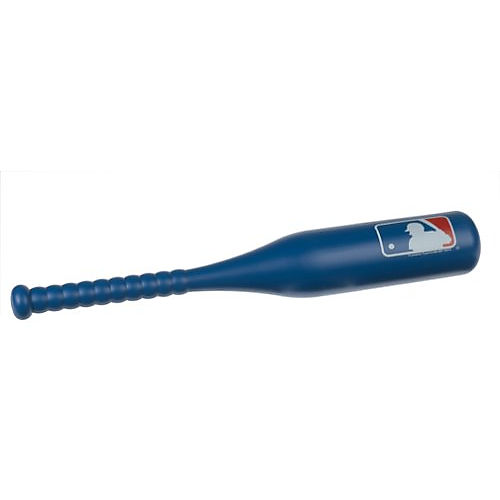
\includegraphics[scale = 0.5]{jumbo_bat.jpg}
\caption{The bat used as an enclosure}
\label{fig:jumbo_bat}
\end{center}
\end{figure}
\clearpage
\newpage

\begin{figure}[htp]
\begin{center}
\vspace{0.4in}
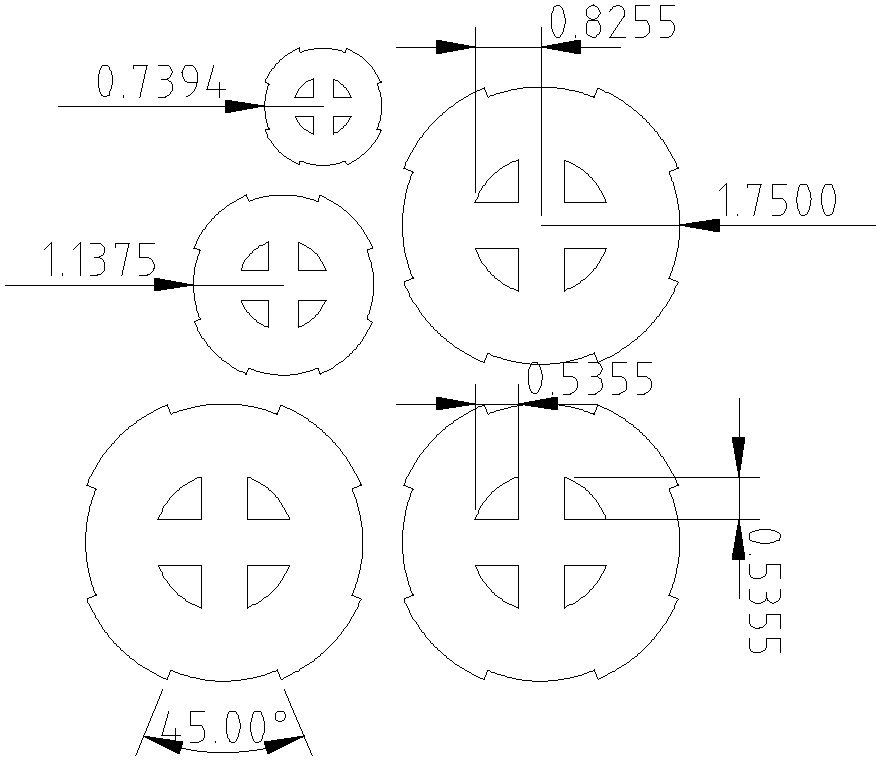
\includegraphics[scale = 0.5]{supports.png}
\caption{CAD design and dimensions for bat internal supports}
\label{fig:supports}
\end{center}
\end{figure}
\clearpage
\newpage

\begin{figure}[htp]
\begin{center}
\vspace{0.4in}
\includegraphics[scale = 0.5]{6uap_hardware_overview.png}
\caption{Hardware Overview}
\label{fig:hardware_overview}
\end{center}
\end{figure}
\clearpage
\newpage

\begin{figure}[htp]
\begin{center}
\vspace{0.4in}
\includegraphics[scale = .75]{6uap_state_machine.png}
\caption{State Machine representation of software}
\label{fig:state_machine}
\end{center}
\end{figure}
\clearpage
\newpage

\begin{figure}[htp]
\begin{center}
\vspace{0.4in}
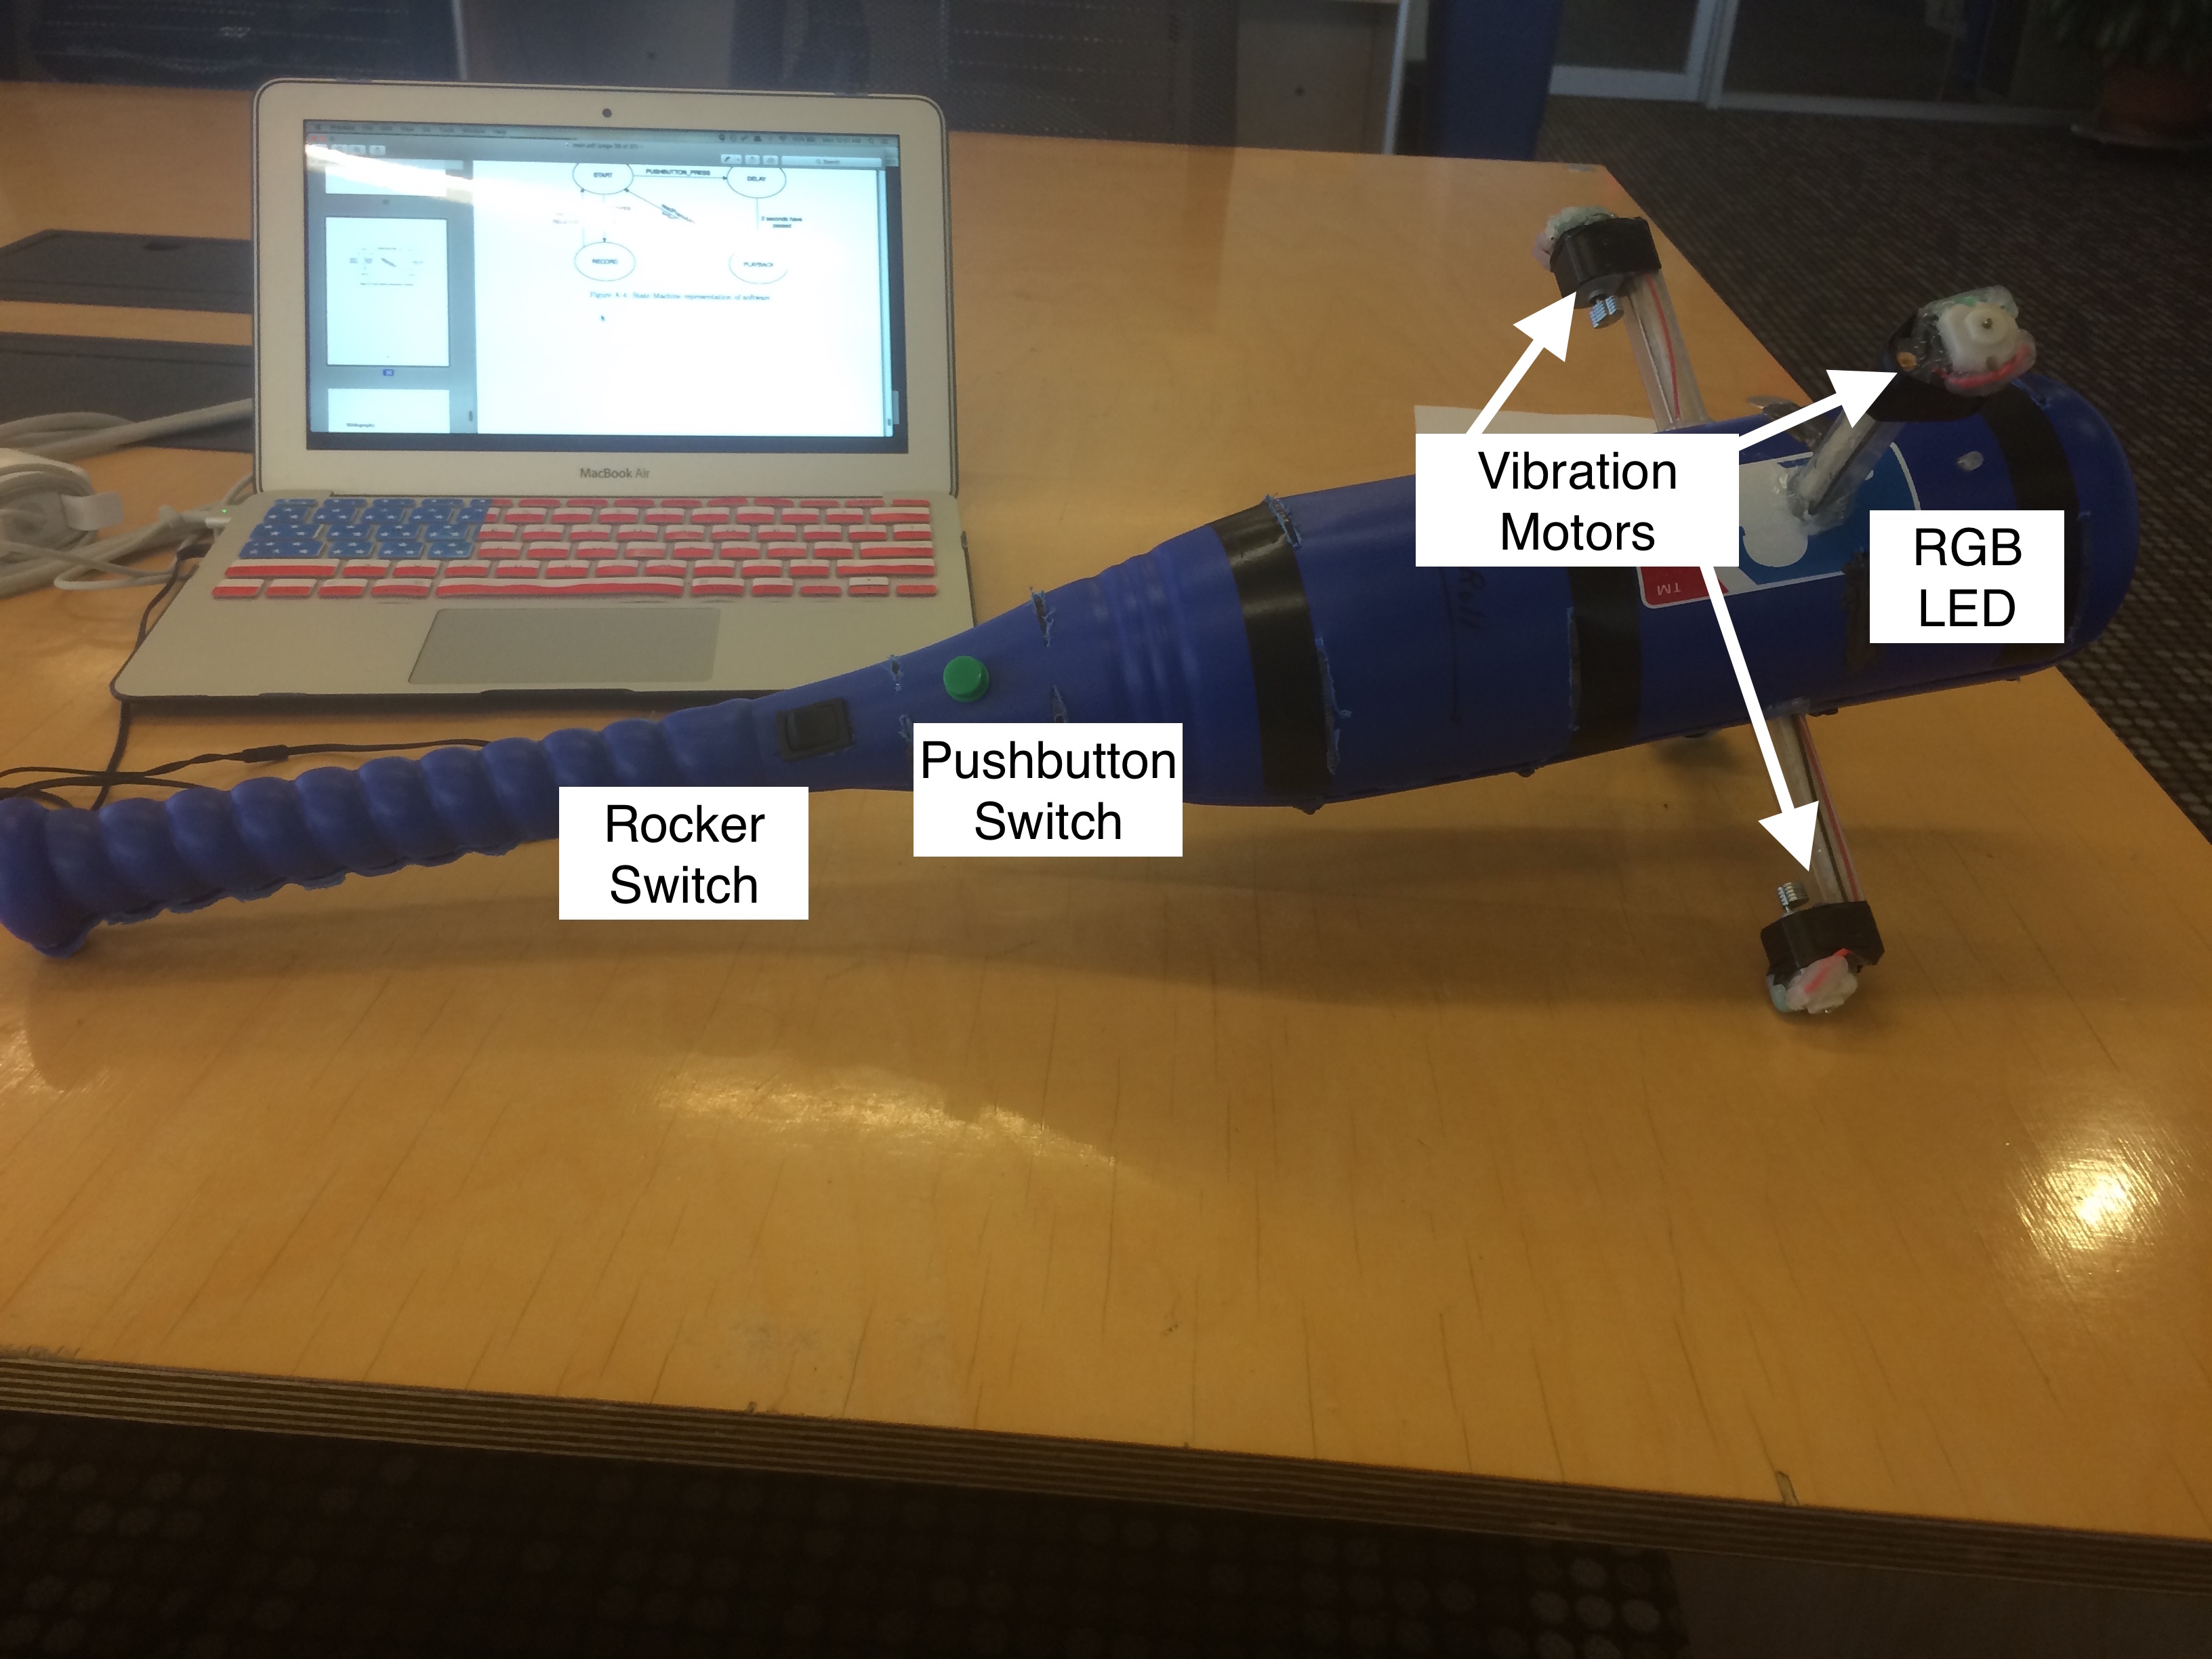
\includegraphics[scale = .12]{bat_front.jpg}
\caption{Outside view of apparatus}
\label{fig:bat_front}
\end{center}
\end{figure}

\begin{figure}[htp]
\begin{center}
\vspace{0.4in}
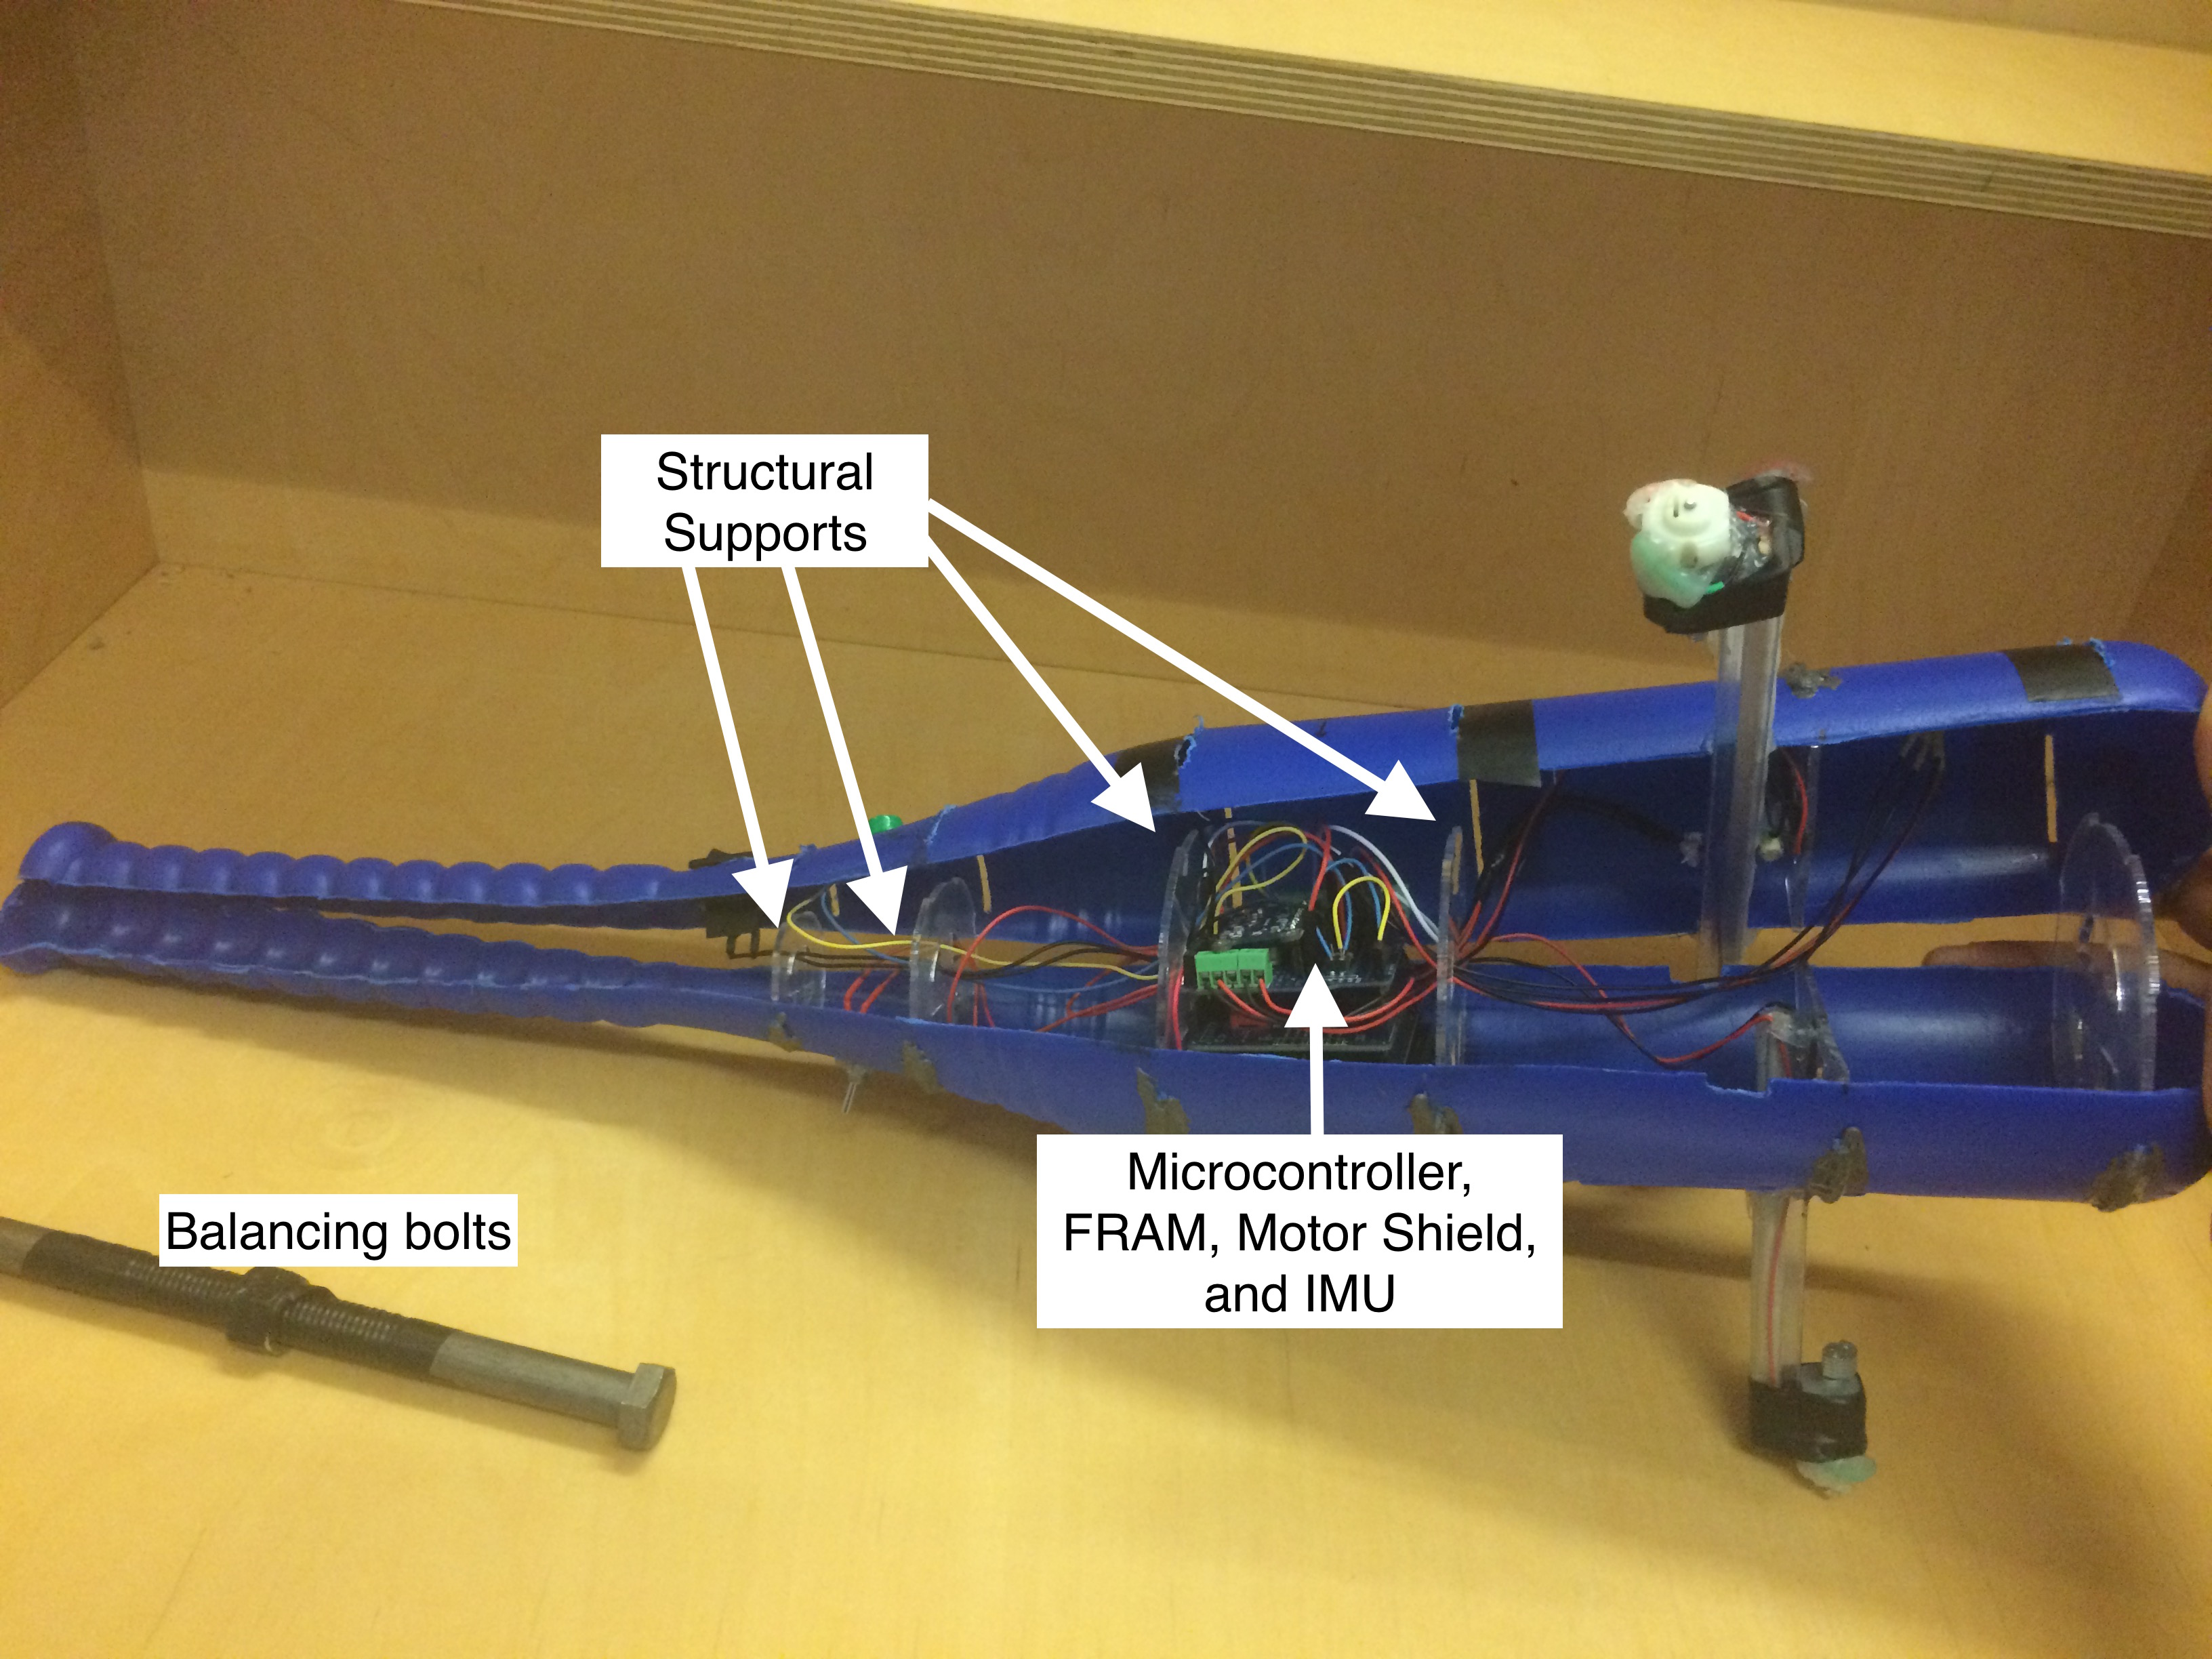
\includegraphics[scale = .12]{bat_inside.jpg}
\caption{Inside of apparatus and hardware}
\label{fig:bat_inside}
\end{center}
\end{figure}
\clearpage
\newpage

%% This defines the bibliography file (main.bib) and the bibliography style.
%% If you want to create a bibliography file by hand, change the contents of
%% this file to a `thebibliography' environment.  For more information 
%% see section 4.3 of the LaTeX manual.
\begin{singlespace}
\bibliography{main}
\bibliographystyle{plain}
\end{singlespace}

\end{document}

